In this section we will describe important design decisions, properties and functionalities of the code generation phase of InSynth.
Afterwards, we will demonstrate the code generation process with an example of code synthesis for a particular input. 

\subsection{Properties of the code generation}

The most important property of the code synthesis is to generate valid code snippets.
Generated code snippets are valid if under an assumption that proof trees obtained from the resolution phase encode valid expressions (and include correct program declarations), the code generation phase synthesises code snippets that, when inserted at the given program point, typecheck to the given type and the overall program compiles successfully.

\subsubsection{Validity of the code generation phase}

Since the code generation phase consists of three steps, we will enumerate their validity properties individually:
\begin{itemize}
\item weighted search - This step performs pruning of initial proof trees in a way that guarantees at least (needed) $N$ expressions to be combined. The pruned proof tree represents a subset of nodes from the original proof tree in such a way that the structure of that subset is preserved, thus the set of expressions encoded in the pruned proof tree must be a subset of set of expressions encoded in the original proof tree.
\item intermediate transform - The correctness of this step directly depends on the correctness of the \textsc{AppAbs} resolution rule and the correspondence between encoded ground types and program declarations. The intermediate transform directly follows the \textsc{AppAbs} rule by transforming, for each provided declaration its parameters according to the enriched context in the case of parameter type being a function or the original context otherwise. Since the transformation is done according to actual program declarations (types), the intermediate transform trees encodes the correct code structure.
\item code snippet generation - This step relies on properties of the target programming language (Scala) and the transformation is defined by programming language syntactic rules and syntactic sugar instances.
\end{itemize} 

\subsubsection{Completeness}

The second important property of the code synthesis is to be complete, in the sense that the code generation phase should generate all expressions that can be found by the resolution phase (i.e. expressed in the target language) and encoded as ``proofs'' in the input InSynth proof trees.

An interesting treatment of the InSynth code synthesis process is the generation of combinators from the SKI combinatory logic
\footnote{many examples in the literature refer to the combinatory logic as SKI, in spite of the fact that combinators S and K provide completeness of the theory, while I can be expressed as I = S K K}.
Combinatory logic may be viewed as a subset of lambda calculus, the theories are largely the same, becoming equivalent in the presence of the rule of extensionality.
Extensional equality captures the mathematical notion of the equality of functions: two functions are equal if they always produce the same results for the same arguments \cite{Tromp:Lambda}.
The SKI combinatory logic contains the same expressive power as lambda calculus and the logic is variable free, i.e. the abstractions are not part of the logic.
Combinators from the SKI combinatory logic can be composed to produce combinators that are extensionally equal to any lambda term, and therefore, by Church's thesis, to any computable function whatsoever.
The process of obtaining an expression in combinatory logic from any given \LC term can be done with the \textit{abstraction elimination} procedure \cite{Tromp:Lambda}.
In the next section we will see that InSynth is capable of synthesis of combinators from the SKI combinatory logic, when the appropriate input type is given.

In our case the extensional equality of two expressions translates to equivalence of behavior of the two expressions under certain evaluation (reduction \cite{Pierce:2002:TPL:509043}) rules.
Although, due to a specific treatment of declarations (which correspond to application terms as defined in \LC) InSynth synthesis process is not capable of producing every possible code snippet that could be otherwise typed by the developer, it can produce a behaviorally (extensionally) equivalent expression, under the reduction rules of the Scala language.
The specific treatment of declarations limit the expressiveness of the application term to an identifier or a declared term - this means that the expression $(\lambda x:Int. x) $ $5$ (where $5$ represents an appropriate \LC encoding of constant 5) which corresponds to Scala code snippet \textit{((x:Int) =\textgreater} \textit{x)(5)} (which typechecks successfully to \textit{Int}) cannot be produced by InSynth, but its behavioral equivalent $(\lambda x:Int. x)[x \rightarrow 5]$ or in Scala, just the literal \textit{5}, can.

We can conclude that InSynth is indeed capable of producing behaviorally equivalent code to every possible Scala expression, thus every reasonable and useful snippet of code.
\footnote{One interesting remark to notice that under some rather strange (and unpractical) reduction rules (like e.g. full beta-reduction \cite{Pierce:2002:TPL:509043}) $(\lambda x:T. y) z$ may not be behaviorally equivalent to $y[x \rightarrow z]$ in all contexts}

Although the code generation phase should be as expressive as the resolution phase resulting proof trees can be (since the code generation phase consults only proof trees for the code extrapolation and synthesis) the intermediate representation adopted provides the same expression power as \LC (which is Turing-complete \cite{odersky:scala,Pierce:2002:TPL:509043, Tromp:Lambda}) and thus is even more expressible than the proof tree encodings.

\subsection{Demonstration example}

We will give an example of InSynth tool code generation process\footnote{such an example seems the most appropriate since the full integration of the code generation module was not yet possible at the time of writing this paper}, show its intermediate outputs and final results, for the case of the $S$ combinator synthesis, somewhat a combinator from the SKI logic \cite{Tromp:Lambda}.
The $S$ combinator is defined as $(S$ $x$ $y$ $z)$ $=$ $(x$ $z$ $(y$ $z))$ and by its nature it does not require any predefined program declarations, i.e. it can be synthesized with the empty program environment.

The Scala declaration with type of the $S$ combinator (instantiated appropriately with Scala primitive types \textit{Int, Char, String} to be able to be represented as a \textit{ground type}) can be given as

\begin{figure}[ht]
\centering
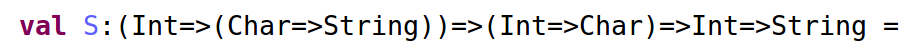
\includegraphics[width=0.45\textwidth]{s_komb}
\end{figure} 

The resulting proof tree as the output of the resolution phase is given in the following figure and it represents nested applications of terms introduced in the context (by the \textsc{AppAbs} rule).

\begin{figure}[ht]
\centering
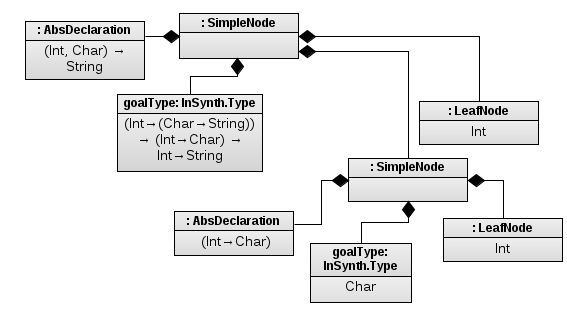
\includegraphics[width=0.40\textwidth]{sav_prez/s_komp_proof_tree}
\end{figure} 

In this particular example the weighted search phase does not affect the tree since there is only one valid expression to be synthesized. 
The intermediate transformation phase produces a tree that in this case completely corresponds to the \LC encoding of the $S$ combinator.

\begin{figure}[ht]
\centering
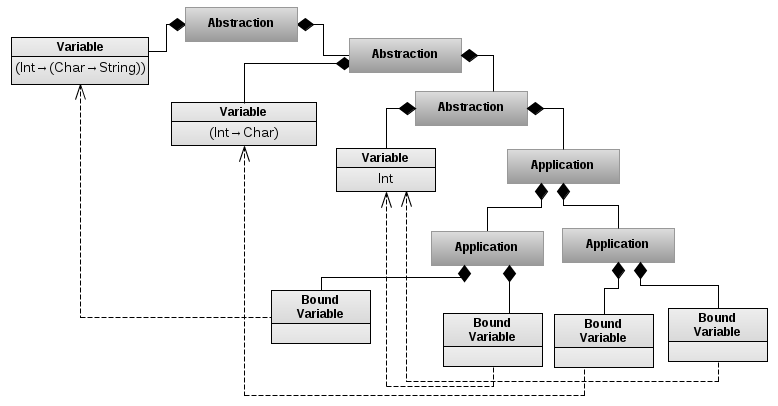
\includegraphics[width=0.45\textwidth]{sav_prez/s_comb_itnermediate}
\end{figure} 

The last step produces of the generation phase produces the scala code which successfully typechecks when inserted as the definition of the declared value \textit{S}. 

\begin{figure}[ht]
\centering
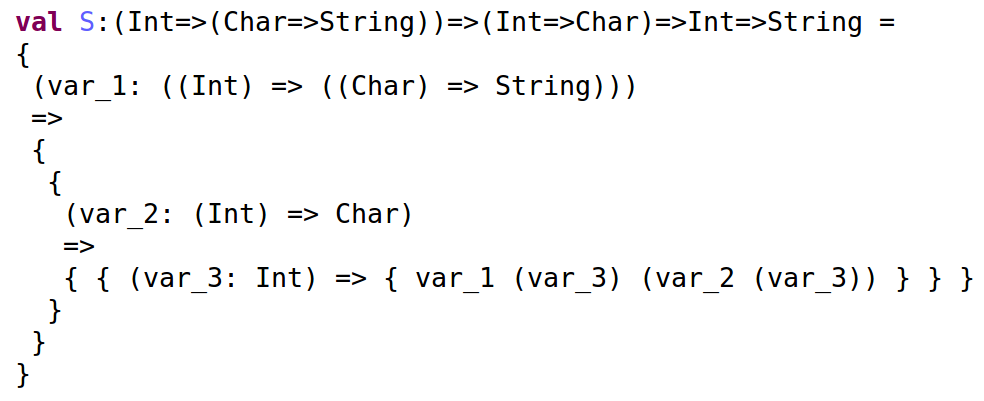
\includegraphics[width=0.45\textwidth]{s_comb_synthesized}
\end{figure} 
